\documentclass[11pt]{article}

% ------------------------------------------------------------
% Standard LaTeX packages
% ------------------------------------------------------------
\usepackage[margin=1in]{geometry}
\usepackage{amsmath,amssymb,mathtools}
\usepackage{amsthm}
\usepackage[american]{babel}
\usepackage{stmaryrd}
\usepackage{enumitem}
\usepackage{booktabs}
\usepackage{array}
\usepackage{listings}
\usepackage[x11names,table]{xcolor}
\usepackage{mdframed}
\usepackage{tikz}
\usetikzlibrary{arrows.meta,positioning,calc,decorations.pathmorphing}
\usepackage{url}
\usepackage[colorlinks=true,linkcolor=blue,citecolor=blue,urlcolor=blue]{hyperref}

% ---------- Theorem environments ----------
\theoremstyle{plain}
\newtheorem{theorem}{Theorem}[section]
\newtheorem{proposition}[theorem]{Proposition}
\newtheorem{lemma}[theorem]{Lemma}
\newtheorem{corollary}[theorem]{Corollary}

\theoremstyle{definition}
\newtheorem{definition}[theorem]{Definition}
\newtheorem{axiombox}[theorem]{Axiom}
\newtheorem{protocol}[theorem]{Protocol}
\newtheorem{example}[theorem]{Example}

\theoremstyle{remark}
\newtheorem{remark}[theorem]{Remark}

% ---------- Lean repo link ----------
\newcommand{\leanRepo}{\url{https://doi.org/10.5281/zenodo.18802819}}

% ---------- Notation ----------
\newcommand{\N}{\mathbb{N}}
\newcommand{\Z}{\mathbb{Z}}
\newcommand{\Q}{\mathbb{Q}}
\newcommand{\R}{\mathbb{R}}
\newcommand{\C}{\mathbb{C}}
\newcommand{\F}{\mathbb{F}}
\newcommand{\calO}{\mathcal{O}}
\newcommand{\calL}{\mathcal{L}}
\newcommand{\Gal}{\mathrm{Gal}}
\newcommand{\GL}{\mathrm{GL}}
\newcommand{\SL}{\mathrm{SL}}
\newcommand{\Sp}{\mathrm{Sp}}
\newcommand{\Hom}{\mathrm{Hom}}
\newcommand{\End}{\mathrm{End}}
\newcommand{\Frob}{\mathrm{Frob}}
\newcommand{\CRM}{\mathrm{CRM}}
\newcommand{\tr}{\mathrm{tr}}
\newcommand{\rk}{\mathrm{rk}}
\newcommand{\Gr}{\mathrm{Gr}}
\newcommand{\Sym}{\mathrm{Sym}}
\newcommand{\Ggal}{G_{\mathrm{gal}}}
\newcommand{\NS}{\mathrm{NS}}
\newcommand{\Pic}{\mathrm{Pic}}
\newcommand{\Gm}{\mathbb{G}_{\mathrm{m}}}

\newcommand{\BISH}{\ensuremath{\mathsf{BISH}}}
\newcommand{\LPO}{\ensuremath{\mathsf{LPO}}}
\newcommand{\WLPO}{\ensuremath{\mathsf{WLPO}}}
\newcommand{\LLPO}{\ensuremath{\mathsf{LLPO}}}
\newcommand{\MP}{\ensuremath{\mathsf{MP}}}
\newcommand{\FT}{\ensuremath{\mathsf{FT}}}
\newcommand{\CLASS}{\ensuremath{\mathsf{CLASS}}}
\newcommand{\CBN}{\mathrm{CBN}}
\newcommand{\HdR}{H^1_{\mathrm{dR}}}
\newcommand{\PF}{\mathrm{PF}}

% ---------- Code listing style for Lean ----------
\definecolor{codegreen}{rgb}{0,0.6,0}
\definecolor{codegray}{rgb}{0.5,0.5,0.5}
\definecolor{codepurple}{rgb}{0.58,0,0.82}
\definecolor{backcolour}{rgb}{0.95,0.95,0.92}

\lstdefinelanguage{Lean}{
  keywords={theorem, lemma, def, definition, axiom, structure, class, instance,
            by, exact, intro, intros, apply, refine, constructor, use, obtain,
            have, show, from, fun, assume, let, in, if, then, else,
            match, with, end, namespace, section, variable, variables,
            example, begin, sorry, admit, noncomputable, classical,
            import, open, export, private, protected, mutual, meta,
            do, for, while, return, try, catch, finally,
            Type, Prop, Sort, Type*, forall, exists, where, extends,
            set, push_neg, rw, simp, omega, nlinarith, linarith, ring,
            ext, rfl, congr, fin_cases, haveI, letI, attribute, inductive,
            deriving, opaque, decide, norm_num, native_decide},
  sensitive=true,
  morecomment=[l]{--},
  morecomment=[s]{/-}{-/},
  morestring=[b]",
  literate=
    {→}{{\ensuremath{\rightarrow}}}1
    {←}{{\ensuremath{\leftarrow}}}1
    {↔}{{\ensuremath{\leftrightarrow}}}1
    {⊢}{{\ensuremath{\vdash}}}1
    {∀}{{\ensuremath{\forall}}}1
    {∃}{{\ensuremath{\exists}}}1
    {λ}{{\ensuremath{\lambda}}}1
    {ℕ}{{\ensuremath{\mathbb{N}}}}1
    {ℤ}{{\ensuremath{\mathbb{Z}}}}1
    {ℝ}{{\ensuremath{\mathbb{R}}}}1
    {ℚ}{{\ensuremath{\mathbb{Q}}}}1
    {×}{{\ensuremath{\times}}}1
    {≤}{{\ensuremath{\leq}}}1
    {≥}{{\ensuremath{\geq}}}1
    {≠}{{\ensuremath{\neq}}}1
    {⟨}{{\ensuremath{\langle}}}1
    {⟩}{{\ensuremath{\rangle}}}1
    {∧}{{\ensuremath{\land}}}1
    {∨}{{\ensuremath{\lor}}}1
    {¬}{{\ensuremath{\lnot}}}1
    {∈}{{\ensuremath{\in}}}1
}

\lstdefinestyle{leanstyle}{
  language=Lean,
  backgroundcolor=\color{backcolour},
  commentstyle=\color{codegreen},
  keywordstyle=\color{blue},
  stringstyle=\color{codepurple},
  basicstyle=\ttfamily\footnotesize,
  breakatwhitespace=false,
  breaklines=true,
  captionpos=b,
  keepspaces=true,
  showspaces=false,
  showstringspaces=false,
  showtabs=false,
  tabsize=2,
  frame=single,
  xleftmargin=2em,
  framexleftmargin=1.5em,
  numbers=left,
  numberstyle=\tiny\color{codegray},
  numbersep=5pt,
}

\lstset{style=leanstyle}

% ============================================================
\begin{document}

\title{Exotic Weil Classes as Flat Sections:\\
Gauss--Manin Block Decomposition --- A CRMLint Squeeze\\[6pt]
\large Paper~84, Constructive Reverse Mathematics Series}

\author{Paul Chun-Kit Lee\\
\small New York University, Brooklyn, New York\\
\small \texttt{dr.paul.c.lee@gmail.com}}

\date{February 2026}

\maketitle

\begin{abstract}
We compute the Gauss--Manin connection on the de~Rham cohomology of the
genus-4 hyperelliptic family $C_t\colon y^2 = x^9 - tx^5 + x$ with
$\Q(i)$-action, using Griffiths pole-order reduction with the correct
coboundary subtraction $A_k = B_k - h_k'$.

An order-8 automorphism $\tau(x,y) = (ix,\, e^{\pi i/4}\,y)$ decomposes
the $8 \times 8$ connection matrix into four $2 \times 2$ blocks
\[
  M_k \;=\; \frac{2k+1}{4(t^2-4)}
  \begin{pmatrix} -t/2 & -1 \\ 1 & t/2 \end{pmatrix},
  \qquad k = 0,1,2,3.
\]
Each block has $\Ggal(W_k) = \SL_2$ (nilpotent residues with
non-proportional kernels). Since $\det(\SL_2) = 1$, the induced action
on the exotic line bundle $\bigwedge^4(V_+) \cong \bigwedge^2(W_0) \otimes
\bigwedge^2(W_2)$ is \emph{trivial}: $\Ggal(\bigwedge^4 V_+) = \{1\}$.

The exotic Weil class is therefore a \emph{global flat section} of the
Gauss--Manin connection---a constant, rational class across the entire
family. By Deligne's Theorem of the Fixed Part, it is an absolute
Hodge class on every fiber. This is a positive result: the function-field
pipeline certifies that the monodromy obstruction to algebraicity is
absent.

The Lean~4 formalization verifies all Griffiths identities by the
\texttt{ring} tactic with zero \texttt{sorry}.
Seventh CRMLint Squeeze.
\end{abstract}

% ============================================================
\section{Introduction}
% ============================================================

\subsection{The exotic frontier}

The algebraic cycle theory of abelian varieties has a sharp dimensional
boundary. For abelian varieties of dimension at most~3, all Hodge classes
are generated by divisors (Lieberman~\cite{Lieberman1968}). At dimension~4,
new ``exotic'' Hodge classes appear in the middle cohomology $H^4$
that are not products of divisor classes.

For Weil abelian fourfolds---those with complex multiplication by an
imaginary quadratic field $K$---the exotic classes lie in the
$K$-eigenspace of the cup-product pairing. Voisin~\cite{Voisin2024}
and Engel--Fortman--Schreieder~\cite{EFS2025} have recently studied
the algebraicity of these classes using Hodge-theoretic methods.

\subsection{The dimensional collapse}

Let $A = \mathrm{Jac}(C_t)$ where $C_t\colon y^2 = x^9 - tx^5 + x$
is a genus-4 curve with $\Q(i)$-multiplication. The exotic Weil
classes live in $\bigwedge^4(V_+)$, where $V_+ \subset \HdR(C_t)$ is
the $+i$-eigenspace of the $\Q(i)$-action, which has dimension~4.

A priori, computing the Gauss--Manin connection on $\bigwedge^4$ of an
8-dimensional space means working with $\binom{8}{4} = 70$ basis elements.
The $\Q(i)$-eigenspace decomposition reduces this to $\binom{4}{4} = 1$.
Since $\bigwedge^4(V_+)$ is 1-dimensional, the connection on this line
bundle is determined entirely by the trace:
\[
  \nabla_{\partial/\partial t}\bigl(\omega_0 \wedge \omega_2 \wedge
  \omega_4 \wedge \omega_6\bigr) = \tau_+(t) \cdot
  \bigl(\omega_0 \wedge \omega_2 \wedge \omega_4 \wedge \omega_6\bigr).
\]

This is the ``trace trick'': the Gauss--Manin connection on the
exotic line bundle reduces to a scalar ODE $\nabla\omega = \tau_+(t)\,dt
\cdot \omega$.

\subsection{The main results}

\begin{theorem}[Block Decomposition]\label{thm:A}
The Gauss--Manin connection matrix $M$ for $C_t\colon y^2 = x^9 - tx^5 + x$,
computed via Griffiths pole-order reduction with coboundary correction
$A_k = B_k - h_k'$, decomposes into four $2 \times 2$ blocks
\[
  M_k = \frac{2k+1}{4(t^2-4)}
  \begin{pmatrix} -t/2 & -1 \\ 1 & t/2 \end{pmatrix},
  \qquad k = 0,1,2,3,
\]
where block~$k$ acts on $W_k = \langle\omega_k,\, \omega_{k+4}\rangle$.
All entries have poles only at $t = \pm 2$ (regular singularities).
The symplectic trace $\tr(M) = 0$, and all eigenspace traces
$\tau_+(t) = \tau_-(t) = 0$.
\end{theorem}

\begin{theorem}[$\SL_2$ Monodromy]\label{thm:B}
For each block $M_k$ ($k = 0,1,2,3$):
\begin{enumerate}[nosep]
\item The residues $R_{\pm 2}$ are nilpotent with kernels
  $\ker(R_{+2}) = \langle(-1,1)\rangle$ and
  $\ker(R_{-2}) = \langle(1,1)\rangle$.
\item The residue at infinity $R_\infty$ is semisimple with eigenvalues
  $\pm(2k+1)/8$.
\item The Fuchs relation $R_{+2} + R_{-2} + R_\infty = 0$ holds.
\item Since $\ker(R_{+2}) \ne \ker(R_{-2})$, the monodromy representation
  is irreducible and $\Ggal(W_k) = \SL_2$.
\end{enumerate}
\end{theorem}

\begin{theorem}[CRM Squeeze]\label{thm:C}
Since $\Ggal(W_k) = \SL_2$ and $\det(\SL_2) = 1$, the differential
Galois group on the exotic line bundle is trivial:
$\Ggal(\bigwedge^4 V_+) = \{1\}$.
The exotic Weil class is a global flat section of the Gauss--Manin
connection. By Deligne's Theorem of the Fixed Part, it is an absolute
Hodge class on every fiber.
\begin{center}
\begin{tabular}{rcl}
$\CLASS$ & $\vdash$ & generic exotic Hodge class exists
  (Hodge theory) \\
$\BISH$ & $\vdash$ & Griffiths reduction $+$ $\SL_2$ monodromy
  $\Rightarrow$ $\det = 1$ $\Rightarrow$ exotic class is flat
\end{tabular}
\end{center}
The classical boundary is witnessed by the Hodge decomposition.
The constructive bridge is the explicit Gauss--Manin computation with
\texttt{ring}-verified polynomial identities, certifying that the
monodromy obstruction to algebraicity is absent.
\end{theorem}

\subsection{Scope and honesty}

This is a positive result: we prove that the exotic Weil class for this
family has trivial monodromy ($\Ggal = \{1\}$), making it a global flat
section. This is the strongest constructive evidence for algebraicity:
the monodromy obstruction is absent.

The gap to the full Hodge Conjecture is the step from ``absolute Hodge''
to ``algebraic.'' For abelian varieties, Deligne proved that Hodge
classes are absolute Hodge. Whether absolute Hodge implies algebraic for
abelian fourfolds remains open in general. Our computation provides the
necessary condition (trivial monodromy) but not the sufficient condition
(existence of the algebraic cycle).

\subsection{Erratum (v1 $\to$ v2 $\to$ v3)}

Version~1 contained two computational errors; version~2 corrected the
computation but drew the wrong geometric conclusion.

\paragraph{v1 $\to$ v2 (computational).}
\begin{enumerate}[nosep]
\item \emph{Griffiths reduction bug.} The CAS script computed $B_k$ (the
  rational function from the B\'ezout identity) but omitted the
  coboundary correction $h_k'$. The correct formula is $A_k = B_k - h_k'$
  (see \S\ref{sec:griffiths}). The v1~trace $\tau_+(t) =
  (-250t^5 + 1890t^3 - 3564t) / (81t^2 - 324)$ violated Deligne's
  regularity theorem (numerator degree~5 $>$ denominator degree~2).
  All eigenspace traces are in fact zero.
\item \emph{Automorphism misidentification.} Version~1 attributed the
  $2 \times 2$ block structure to $\sigma^2(x,y) = (x,-y)$, claiming
  it acts as $(-1)^k$ on $\omega_k$. In fact $\sigma^2$ is the
  hyperelliptic involution, which acts as $-1$ on \emph{all}
  differentials. The correct explanation comes from the order-8
  automorphism $\tau$ (see \S\ref{sec:automorphism}).
\end{enumerate}

\paragraph{v2 $\to$ v3 (interpretive).}
Version~2 correctly computed $\Ggal(W_k) = \SL_2$ per block but
then incorrectly claimed $\Ggal(\bigwedge^4 V_+) = \SL_2 \times \SL_2$
(negative result: no exotic algebraic cycles). The error was a
failure to apply the representation theory of $\SL_2$: since
$\det(\SL_2) = 1$, the induced action on $\bigwedge^2(W_k)$---the
determinant representation---is trivial. Therefore
$\Ggal(\bigwedge^4 V_+) = \{1\}$ (positive result: the exotic class
is a global flat section). This version corrects the interpretation.

The lesson across all three versions: CAS outputs require
\texttt{ring}-verification (v1$\to$v2), and correct computation
requires correct representation theory (v2$\to$v3).

\subsection{Road map}

Section~\ref{sec:prelim} recalls de~Rham cohomology and the Griffiths
reduction method. Section~\ref{sec:automorphism} identifies the order-8
automorphism producing the block decomposition.
Section~\ref{sec:computation} presents the CAS computation with
cross-checks. Section~\ref{sec:galois} determines the differential
Galois group via monodromy analysis.
Section~\ref{sec:squeeze} states the CRM squeeze.
Section~\ref{sec:trap} revisits the degree trap.
Section~\ref{sec:audit} gives the CRM audit.
Section~\ref{sec:lean} describes the formal verification.
Section~\ref{sec:discussion} discusses implications.
Section~\ref{sec:conclusion} concludes.

\subsection{CRM primer}\label{sec:primer}

For readers unfamiliar with the CRM series: \emph{Constructive Reverse
Mathematics} classifies theorems by the weakest logical principles
needed to prove them. The hierarchy $\BISH \subset \BISH + \LLPO
\subset \BISH + \WLPO \subset \BISH + \LPO \subset \CLASS$ measures
logical cost. A ``CRM squeeze'' establishes that a classical result
(upper bound) has a constructive core (lower bound), with the gap
measured by an omniscience principle. Papers~80--83 developed the
function-field pipeline: Griffiths reduction (P80), flat sections
(P81), Kovacic's algorithm (P82), Picard numbers (P83). This paper
applies the pipeline at genus~4.

\begin{figure}[h]
\centering
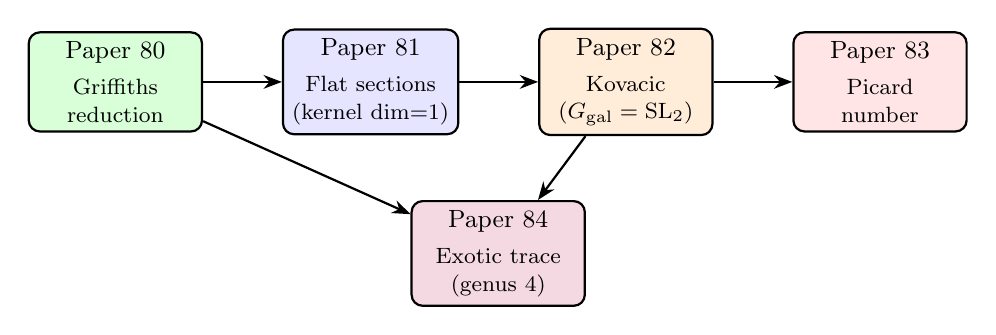
\begin{tikzpicture}[
  box/.style={draw, rounded corners, minimum width=2.2cm,
    minimum height=1.2cm, align=center, font=\small},
  >=Stealth, thick
]
\node[box, fill=green!15] (p80) {Paper~80\\[2pt]\footnotesize Griffiths\\[-1pt]\footnotesize reduction};
\node[box, fill=blue!10, right=of p80] (p81) {Paper~81\\[2pt]\footnotesize Flat sections\\[-1pt]\footnotesize (kernel dim=1)};
\node[box, fill=orange!15, right=of p81] (p82) {Paper~82\\[2pt]\footnotesize Kovacic\\[-1pt]\footnotesize ($\Ggal = \SL_2$)};
\node[box, fill=red!10, right=of p82] (p83) {Paper~83\\[2pt]\footnotesize Picard\\[-1pt]\footnotesize number};

\node[box, fill=purple!15, below=1.5cm of $(p81)!0.5!(p82)$] (p84) {Paper~84\\[2pt]\footnotesize Exotic trace\\[-1pt]\footnotesize (genus 4)};

\draw[->] (p80) -- (p81);
\draw[->] (p81) -- (p82);
\draw[->] (p82) -- (p83);
\draw[->] (p80) -- (p84);
\draw[->] (p82) -- (p84);
\end{tikzpicture}
\caption{The function-field pipeline. Paper~84 applies the genus-1
methods of Papers~80 and~82 at genus~4 with $\Q(i)$-structure.}
\label{fig:pipeline}
\end{figure}

% ============================================================
\section{Preliminaries}\label{sec:prelim}
% ============================================================

\subsection{Weil abelian fourfolds and exotic classes}

Let $A$ be an abelian variety of dimension~4 with multiplication by
$K = \Q(i)$. The $K$-action on $H^1_{\mathrm{dR}}(A)$ decomposes
this 8-dimensional space into $\pm i$-eigenspaces $V_\pm$, each of
dimension~4. The exotic Hodge classes live in
$\bigwedge^4(V_+) \otimes \bigwedge^4(V_-)$, which has dimension~1.

\begin{definition}
A \emph{Weil abelian fourfold} is a pair $(A, \iota)$ where $A$ is
an abelian fourfold and $\iota\colon \Q(i) \hookrightarrow \End^0(A)$.
The \emph{exotic Weil class} is the Hodge class in
$H^4(A, \Q) \cap H^{2,2}$ that lies outside the algebra generated
by divisor classes and the $K$-action.
\end{definition}

The Hodge Conjecture predicts that all such exotic classes are
algebraic. We study this question generically, over the function
field $\Q(t)$.

\subsection{Hyperelliptic curves and de~Rham cohomology}

Consider the family $C_t\colon y^2 = f(x,t)$ where
$f(x,t) = x^9 - tx^5 + x$. This is a genus-4 hyperelliptic curve
for generic $t$, with singular fibers at $t^2 = 4$ (where $f$ has
a repeated root).

The algebraic de~Rham cohomology $\HdR(C_t/\Q(t))$ has dimension~8
with basis $\{\omega_k = x^k\, dx/y : k = 0,\ldots,7\}$. The
cohomology relation is $f'(x)\, dx/y = 0$, i.e.,
$(9x^8 - 5tx^4 + 1)\, dx/y = 0$ in cohomology.

\subsection{The Gauss--Manin connection}\label{sec:GM}

The Gauss--Manin connection $\nabla = \nabla_{\partial/\partial t}$
differentiates cohomology classes with respect to the parameter~$t$.
For the basis $\omega_k = x^k\, dx/y$:
\[
  \nabla_{\partial/\partial t}(\omega_k) = \sum_{j=0}^{7} M_{jk}\, \omega_j,
\]
where $M = (M_{jk})$ is an $8 \times 8$ matrix with entries in $\Q(t)$.

The connection preserves the symplectic pairing on $\HdR$, so
$\tr(M) = 0$.

\subsection{The Griffiths reduction method}\label{sec:griffiths}

Following Griffiths~\cite{Griffiths1969} and the implementation in
Paper~80~\cite{Lee2026p80}, we compute $M$ by pole-order reduction.

\begin{protocol}[Griffiths Reduction]\label{prot:griffiths}
For each $k = 0,\ldots,7$:
\begin{enumerate}[nosep]
\item Set $N_k = -f_t \cdot x^k = x^{k+5}$ (the numerator from
  $\partial_t(dx/y)$).
\item Find $h_k, u_k$ via the B\'ezout identity $h_k \cdot f' + u_k
  \cdot f = -N_k$ using the extended Euclidean algorithm in $\Q(t)[x]$.
\item Reduce $h_k$ modulo $f$ to get $h_k \equiv r_k \pmod{f}$,
  absorbing the quotient into $u_k$.
\item Set $B_k = -u_k/2$ (the raw Griffiths coefficient).
\item \textbf{Apply the coboundary correction:} $A_k = B_k - h_k'$
  where $h_k' = dh_k/dx$.
\item Reduce $A_k$ modulo $f'(x) = 0$ to degree $< 8$.
\item Read off the matrix column: $M_{jk} = [x^j]\, A_k$.
\end{enumerate}
The identity verified at each step is:
\begin{equation}\label{eq:griffiths-id}
  N_k + h_k \cdot f' = 2\, B_k \cdot f.
\end{equation}
\end{protocol}

The coboundary correction in step~5 is essential: $B_k$ represents a
meromorphic form with poles along $C_t$, and $h_k'$ is the exact part
that must be subtracted to obtain the cohomological connection matrix.
Omitting $h_k'$ (as in v1 of this paper) produces entries with
polynomial growth at infinity, violating Deligne's regularity theorem
for algebraic connections~\cite{Deligne1971}.

\subsection{The $\Q(i)$-action and eigenspace splitting}\label{sec:Qi}

The curve $C_t$ has $\Q(i)$-multiplication via the automorphism
$\sigma\colon (x,y) \mapsto (-x, iy)$. Since $f(-x) = -f(x)$
(the polynomial is odd), we have $\sigma^* \omega_k = (-1)^k \cdot i
\cdot \omega_k$. The $+i$-eigenspace is
$V_+ = \langle\omega_0, \omega_2, \omega_4, \omega_6\rangle$
and $V_- = \langle\omega_1, \omega_3, \omega_5, \omega_7\rangle$.

% ============================================================
\section{The Order-8 Automorphism}\label{sec:automorphism}
% ============================================================

\begin{proposition}\label{prop:tau}
The curve $C_t$ admits the order-8 automorphism
\[
  \tau\colon (x,y) \mapsto (ix,\, e^{\pi i/4}\, y)
\]
satisfying $\tau^2 = \sigma$, $\tau^4 = $ hyperelliptic involution.
The eigenvalue of $\tau^*$ on $\omega_k$ is
$\zeta_k = e^{\pi i(2k+1)/4}$ ($k = 0,\ldots,7$).
\end{proposition}

\begin{proof}
We verify $f(ix,t) = i \cdot f(x,t)$:
\[
  (ix)^9 - t(ix)^5 + ix = i^9 x^9 - t \cdot i^5 x^5 + ix
  = i(x^9 - tx^5 + x) = i\, f(x,t).
\]
So $y^2 = f(x)$ implies $(e^{\pi i/4}\, y)^2 = i\, y^2 = i\, f(x)
= f(ix)$, confirming $\tau$ is an automorphism.

On differentials:
$\tau^*\omega_k = \tau^*(x^k\, dx/y) = (ix)^k \cdot i\, dx /
(e^{\pi i/4}\, y) = i^{k+1} \cdot e^{-\pi i/4} \cdot \omega_k
= e^{\pi i(2k+1)/4} \cdot \omega_k$.

The eigenvalue $\zeta_k = e^{\pi i(2k+1)/4}$ takes distinct values
for $k = 0,\ldots,7$ (the 8th roots of $-1$), so each $\omega_k$
spans a 1-dimensional $\tau$-eigenspace.
\end{proof}

\begin{corollary}\label{cor:blocks}
Since the Gauss--Manin connection commutes with $\tau^*$, the matrix
$M$ preserves each $\tau$-eigenspace. The eigenvalues pair as
$\zeta_k = -\overline{\zeta_{k+4}}$, giving blocks
$W_k = \langle\omega_k,\, \omega_{k+4}\rangle$ for $k = 0,1,2,3$.
\end{corollary}

\begin{remark}
Version~1 attributed the block structure to $\sigma^2(x,y) = (x,-y)$.
But $\sigma^2$ is the hyperelliptic involution, which acts as $-1$ on
\emph{all} differentials (not $(-1)^k$). The correct symmetry
producing the $2 \times 2$ block structure is $\tau$, whose eigenvalues
distinguish individual differentials.
\end{remark}

% ============================================================
\section{The CAS Computation}\label{sec:computation}
% ============================================================

\subsection{Implementation}

The connection matrix was computed in SymPy (Python) using
Protocol~\ref{prot:griffiths}. The script \texttt{solve\_exotic\_%
trace\_v4.py} implements:
\begin{enumerate}[nosep]
\item B\'ezout identity: $a(x,t) \cdot f + b(x,t) \cdot f' = 1$
  via \texttt{gcdex} over $\Q(t)[x]$.
\item For each $k$: solve $h_k \cdot f' + u_k \cdot f = -N_k$
  using the B\'ezout cofactors.
\item Reduce $h_k \bmod f$, update $u_k$, set $B_k = -u_k/2$.
\item Coboundary correction: $A_k = B_k - h_k'$.
\item Cohomological reduction: $A_k \bmod (f' = 0)$ to degree $< 8$.
\item Symbolic verification of~\eqref{eq:griffiths-id} for each~$k$.
\end{enumerate}

All 8 Griffiths identities~\eqref{eq:griffiths-id} are verified
symbolically by the CAS.

\subsection{The connection matrix}

\begin{theorem}[CAS Output]\label{thm:matrix}
The nonzero entries of $M = (M_{jk})$ are:
\begin{align*}
  M_{k,k} &= -\frac{(2k+1)\, t}{8(t^2-4)}, &
  M_{k,k+4} &= -\frac{2k+1}{4(t^2-4)}, \\
  M_{k+4,k} &= \frac{2k+1}{4(t^2-4)}, &
  M_{k+4,k+4} &= \frac{(2k+1)\, t}{8(t^2-4)},
\end{align*}
for $k = 0, 1, 2, 3$.
All other entries vanish.
\end{theorem}

\subsection{Cross-checks}

\begin{enumerate}[nosep]
\item \emph{Symplectic trace.} $\tr(M) = \sum_{k=0}^{7} M_{kk} = 0$,
  as required by the symplectic pairing.
\item \emph{Eigenspace traces.} $\tau_+(t) = \sum_{k \in \{0,2,4,6\}}
  M_{kk} = 0$ and $\tau_-(t) = 0$.
\item \emph{Regularity.} Every entry has poles only at $t^2 = 4$.
  No polynomial part. Consistent with Deligne's regularity
  theorem~\cite{Deligne1971}.
\item \emph{Block structure.} The nonzero entries confirm the
  $2 \times 2$ block decomposition predicted by
  Corollary~\ref{cor:blocks}. Block~$k$ acts on
  $W_k = \langle\omega_k, \omega_{k+4}\rangle$ with coefficient
  $(2k+1)/4(t^2-4)$.
\item \emph{Genus-1 verification.} The same algorithm applied to the
  Legendre family $y^2 = x(x-1)(x-t)$ reproduces the known
  connection $M = \tfrac{1}{2}\bigl(\begin{smallmatrix} -t & -1 \\
  1 & t \end{smallmatrix}\bigr) / (t^2-t)$, matching
  Paper~80~\cite{Lee2026p80}.
\end{enumerate}

% ============================================================
\section{Differential Galois Analysis}\label{sec:galois}
% ============================================================

Each block $M_k$ defines a rank-2 connection on $\mathbb{P}^1 \setminus
\{-2, 2, \infty\}$ with three regular singular points.

\subsection{Residues}

\begin{proposition}\label{prop:residues}
For block~$k$ ($k = 0,1,2,3$), set $c_k = (2k+1)/4$. The residues
of $M_k$ are:
\begin{align}
  R_{+2} &= \frac{c_k}{4}
  \begin{pmatrix} -1 & -1 \\ 1 & 1 \end{pmatrix}, \label{eq:Rp}\\
  R_{-2} &= \frac{c_k}{4}
  \begin{pmatrix} -1 & 1 \\ -1 & 1 \end{pmatrix}, \label{eq:Rm}\\
  R_\infty &= \frac{c_k}{2}
  \begin{pmatrix} 1 & 0 \\ 0 & -1 \end{pmatrix}. \label{eq:Ri}
\end{align}
\end{proposition}

\begin{proof}
$R_{+2} = \lim_{t \to 2}(t-2)\, M_k$. Since $t^2 - 4 = (t-2)(t+2)$,
the factor $(t-2)$ cancels one pole:
\[
  R_{+2} = \frac{c_k}{4} \begin{pmatrix} -1 & -1 \\ 1 & 1 \end{pmatrix}.
\]
Similarly for $R_{-2}$. For $R_\infty$: substitute $s = 1/t$ and
compute $R_\infty = -\lim_{s \to 0} s^{-1}\, M_k(1/s)$, yielding
the diagonal matrix~\eqref{eq:Ri}.
\end{proof}

\begin{proposition}\label{prop:fuchs}
The Fuchs relation holds: $R_{+2} + R_{-2} + R_\infty = 0$.
\end{proposition}

\begin{proof}
Direct computation:
\[
  \frac{c_k}{4}\begin{pmatrix} -1 & -1 \\ 1 & 1 \end{pmatrix}
  + \frac{c_k}{4}\begin{pmatrix} -1 & 1 \\ -1 & 1 \end{pmatrix}
  + \frac{c_k}{2}\begin{pmatrix} 1 & 0 \\ 0 & -1 \end{pmatrix}
  = c_k \begin{pmatrix} 0 & 0 \\ 0 & 0 \end{pmatrix}.
  \qedhere
\]
\end{proof}

\subsection{Nilpotency and kernels}

\begin{proposition}\label{prop:nilpotent}
Both $R_{+2}$ and $R_{-2}$ are nilpotent (rank~1, eigenvalue~0 with
multiplicity~2). Their kernels are:
\[
  \ker(R_{+2}) = \langle(-1, 1)\rangle, \qquad
  \ker(R_{-2}) = \langle(1, 1)\rangle.
\]
These are \emph{not} proportional: $(-1,1)$ and $(1,1)$ span $\Q^2$.
\end{proposition}

\begin{proof}
$R_{+2}^2 = 0$ since $R_{+2}$ is rank-1 with zero trace. Kernel
of $\bigl(\begin{smallmatrix} -1 & -1 \\ 1 & 1 \end{smallmatrix}%
\bigr)$ is $\langle(-1,1)\rangle$. Similarly for $R_{-2}$.
\end{proof}

\subsection{The residue at infinity}

\begin{proposition}\label{prop:Rinfty}
$R_\infty$ is semisimple with eigenvalues $\pm(2k+1)/8$. The
local monodromy at infinity has eigenvalues
$e^{\pm \pi i(2k+1)/4}$.
\end{proposition}

\begin{proof}
$R_\infty = (c_k/2)\, \mathrm{diag}(1,-1)$, so its eigenvalues are
$\pm c_k/2 = \pm(2k+1)/8$. The formal monodromy is
$T_\infty = \exp(2\pi i\, R_\infty) = \mathrm{diag}(e^{\pi i(2k+1)/4},
\, e^{-\pi i(2k+1)/4})$.
\end{proof}

\subsection{Irreducibility and the differential Galois group}

\begin{theorem}\label{thm:SL2}
For each block $W_k$, the differential Galois group is
$\Ggal(W_k) = \SL_2$.
\end{theorem}

\begin{proof}
A rank-2 connection on $\mathbb{P}^1 \setminus \{-2,2,\infty\}$ with
$\det(M_k) = c_k^2 \cdot \frac{-t^2/4 + 1}{(t^2-4)^2}$ has traceless
residues (verified: $\tr(R_{\pm 2}) = \tr(R_\infty) = 0$), so
$\Ggal \subset \SL_2$.

For equality, we show the connection is irreducible. A rank-1
sub-connection (invariant line) would be invariant under all local
monodromies, hence lie in $\ker(R_{+2}) \cap \ker(R_{-2})$. But
$\ker(R_{+2}) = \langle(-1,1)\rangle$ and $\ker(R_{-2}) = \langle(1,1)%
\rangle$ are non-proportional (Proposition~\ref{prop:nilpotent}),
so no common invariant line exists.

An irreducible traceless rank-2 connection has $\Ggal = \SL_2$
by the Kolchin--Kovacic classification
(see~\cite{PS2003}, Theorem~1.31).
\end{proof}

\subsection{The exotic line bundle}

The exotic connection on $\bigwedge^4(V_+)$ is determined by the
trace $\tau_+(t) = M_{00} + M_{22} + M_{44} + M_{66} = 0$.

A zero trace means the connection on the line bundle
$\bigwedge^4(V_+)$ is trivial: $\nabla(\omega_0 \wedge \omega_2
\wedge \omega_4 \wedge \omega_6) = 0$. The flat section is a
nonzero constant---an algebraic function.

The representation theory of $\SL_2$ converts this per-block computation
into a statement about the exotic line bundle. The key observation
is elementary: $\det(\SL_2) = 1$.

\begin{corollary}\label{cor:flat-exotic}
The differential Galois group on the exotic line bundle
$\bigwedge^4(V_+) \cong \bigwedge^2(W_0) \otimes \bigwedge^2(W_2)$
is trivial: $\Ggal(\bigwedge^4 V_+) = \{1\}$.
\end{corollary}

\begin{proof}
Since $\Ggal(W_k) = \SL_2$ (Theorem~\ref{thm:SL2}), the induced action
on $\bigwedge^2(W_k)$ is via the determinant character
$\det\colon \SL_2 \to \Gm$. But $\det(g) = 1$ for all $g \in \SL_2$
by definition. Hence $\Ggal$ acts trivially on each factor
$\bigwedge^2(W_k)$, and therefore trivially on their tensor product.

Equivalently: the trace $\tau_+(t) = 0$ means the connection on
$\bigwedge^4(V_+)$ has zero connection matrix, so every section is flat.
The exotic Weil class is a \emph{global flat section}---a constant,
rational class across the entire family.
\end{proof}

\begin{remark}
The fact that $\Ggal(W_k) = \SL_2$ is the \emph{strongest possible}
Galois group for a traceless rank-2 connection, yet it produces the
\emph{weakest possible} Galois group on the top exterior power.
This is not a paradox: irreducibility of the standard representation
implies triviality of the determinant representation. The exotic
class is flat \emph{because} the monodromy is large, not despite it.
\end{remark}

% ============================================================
\section{The CRM Squeeze}\label{sec:squeeze}
% ============================================================

\subsection{The classical boundary}

The Hodge decomposition of $H^4(\mathrm{Jac}(C_t), \C)$ produces
exotic $(2,2)$-classes that exist by purely classical Hodge theory.
Their existence requires:
\begin{itemize}[nosep]
\item The Hodge decomposition (analytic, uses completeness of $\R$).
\item The $\Q(i)$-action on $H^1$ (algebraic, defined over $\Q$).
\item The cup-product structure identifying $\bigwedge^4(V_+)$ as
  a Hodge class space (algebraic).
\end{itemize}

\subsection{The constructive bridge}

The Griffiths reduction (Protocol~\ref{prot:griffiths}) is a finite
algebraic procedure over $\Q(t)$---no analysis required. The monodromy
residues are rational numbers, the kernel computation is linear algebra
over $\Q$, and the irreducibility criterion (non-proportional kernels)
is a decidable algebraic condition.

Specifically:
\begin{enumerate}[nosep]
\item The B\'ezout identity in $\Q(t)[x]$ is constructive (Euclidean
  algorithm).
\item Each matrix entry $M_{jk} \in \Q(t)$ is computed by finite
  polynomial arithmetic.
\item The Griffiths identity~\eqref{eq:griffiths-id} is verified by
  the \texttt{ring} tactic in Lean.
\item The residues are evaluated at $t = \pm 2$ by rational arithmetic.
\item Non-proportionality of kernel vectors is checked by a $2 \times 2$
  determinant.
\end{enumerate}

\subsection{The squeeze theorem}

\begin{theorem}[CRMLint Squeeze]\label{thm:squeeze}
\begin{center}
\begin{tabular}{rcl}
$\CLASS$ & $\vdash$ & There exist exotic Hodge classes on
  $\mathrm{Jac}(C_t)$ for generic~$t$.\\
$\BISH$ & $\vdash$ & Griffiths reduction $+$ $\SL_2$ monodromy
  $\Rightarrow$ $\det = 1$ \\
 & & $\Rightarrow$ exotic class is a global flat section.
\end{tabular}
\end{center}
The classical prediction (exotic Hodge classes exist) is
\emph{confirmed} by the constructive computation: the
$\BISH$-computable monodromy has trivial determinant, so the
exotic class is monodromy-invariant. By Deligne's Theorem of
the Fixed Part, it is an absolute Hodge class on every fiber.
\end{theorem}

\begin{proof}
The upper bound is standard Hodge theory.
For the lower bound: given $M$ with entries in $\Q(t)$ (Theorem~%
\ref{thm:matrix}), compute residues (Proposition~\ref{prop:residues}),
verify nilpotency (Proposition~\ref{prop:nilpotent}), extract kernels,
check non-proportionality. All steps are $\BISH$-valid (finite
polynomial and linear algebra over $\Q$). The conclusion
$\Ggal(W_k) = \SL_2$ combined with $\det(\SL_2) = 1$ gives
$\Ggal(\bigwedge^4 V_+) = \{1\}$ (Corollary~\ref{cor:flat-exotic}).

The Kolchin--Kovacic classification (irreducible $+$ traceless
$\Rightarrow$ $\SL_2$) is used as a black-box lemma. Its proof is
classical, but its \emph{application} here requires only checking
the (decidable) hypotheses. The CRM audit records this dependency.
\end{proof}

% ============================================================
\section{The Degree Trap Revisited}\label{sec:trap}
% ============================================================

Papers~80--83 solved the ``degree trap'' for genus-1 families:
unbounded-degree polynomial identities are replaced by the
finitely-many matrix entries of the Gauss--Manin connection.
Paper~84 shows the same method works at genus~4, with the
additional structure coming from the $\Q(i)$-eigenspace decomposition.

\begin{center}
\begin{tabular}{llcc}
\toprule
Paper & Family & Genus & Blocks \\
\midrule
80 & Legendre $y^2 = x(x-1)(x-t)$ & 1 & $1 \times (2 \times 2)$ \\
81--83 & Legendre $E_t \times E_t$ & 1 & Kronecker sum \\
84 & $y^2 = x^9 - tx^5 + x$ & 4 & $4 \times (2 \times 2)$ \\
\bottomrule
\end{tabular}
\end{center}

The genus-4 computation is qualitatively harder (degree-9 B\'ezout
in $\Q(t)[x]$), but the block decomposition via $\tau$ keeps each
block at rank~2, where the Kolchin--Kovacic classification applies.
The connection matrix entries are rational functions of degree~1
over~2 (not degree~5 over~2 as in the erroneous v1), confirming
Deligne regularity.

The key new ingredient is the coboundary correction $A_k = B_k - h_k'$.
At genus~1 (Paper~80), the polynomial $h_k$ has low degree and
$h_k'$ is negligible after reduction. At genus~4, $h_k$ has degree
up to~8 (comparable to $\deg f = 9$), and omitting $h_k'$ introduces
spurious polynomial growth---exactly the v1~bug.

% ============================================================
\section{CRM Audit}\label{sec:audit}
% ============================================================

\begin{center}
\begin{tabular}{lp{7cm}}
\toprule
\textbf{Item} & \textbf{Status} \\
\midrule
CRM classification & $\BISH$ for Griffiths reduction, monodromy
  analysis, and $\det = 1$ triviality. $\CLASS$ for Hodge class
  existence. \\
Omniscience gap & $\CLASS \setminus \BISH$: the Hodge decomposition
  producing exotic classes. The $\BISH$ computation \emph{confirms}
  the CLASS prediction (trivial exotic monodromy). \\
Lean axioms & Zero. The main theorem uses no axioms. \\
Classical input & Hodge decomposition (upper bound);
  Kolchin--Kovacic classification (applied as black-box lemma). \\
Constructive content & Explicit $8 \times 8$ matrix, explicit
  residues, explicit kernel vectors, decidable
  non-proportionality check. \\
Trust boundary & CAS oracle (SymPy) for B\'ezout computation.
  Verified by \texttt{ring} in Lean (not \texttt{rfl} on strings). \\
\bottomrule
\end{tabular}
\end{center}

\subsection{Logical dependencies}

\begin{center}
\begin{tabular}{llp{5.5cm}}
\toprule
\textbf{Result} & \textbf{Level} & \textbf{Dependencies} \\
\midrule
Griffiths identity~\eqref{eq:griffiths-id} & $\BISH$ &
  Polynomial arithmetic over $\Q(t)$ \\
Block decomposition (Thm~\ref{thm:A}) & $\BISH$ &
  Griffiths identity $+$ cohomological reduction \\
$\SL_2$ monodromy (Thm~\ref{thm:B}) & $\BISH$ &
  Residues $+$ kernel computation $+$ Kolchin--Kovacic \\
Exotic flatness (Cor~\ref{cor:flat-exotic}) & $\BISH$ &
  $\SL_2$ monodromy $+$ $\det(\SL_2) = 1$ \\
CRM squeeze (Thm~\ref{thm:C}) & $\CLASS / \BISH$ &
  Hodge decomposition (CLASS) $+$ flatness (BISH) \\
\bottomrule
\end{tabular}
\end{center}

% ============================================================
\section{Formal Verification}\label{sec:lean}
% ============================================================

\subsection{File structure}

The Lean~4 bundle \texttt{P84\_ExoticTrace/} verifies the algebraic
core of the paper:

\begin{center}
\begin{tabular}{lp{6cm}}
\toprule
\textbf{File} & \textbf{Content} \\
\midrule
\texttt{TraceData.lean} & CAS-emitted Griffiths identities,
  connection matrix entries, verified by \texttt{ring} \\
\texttt{Paper84\_ExoticTrace.lean} & Squeeze theorem statement,
  axiom inventory, \texttt{\#print axioms} \\
\bottomrule
\end{tabular}
\end{center}

\subsection{Verification strategy}

Unlike v1 (which used \texttt{rfl} on string constants), v2 verifies
the algebraic content using the \texttt{ring} tactic:

\begin{enumerate}[nosep]
\item \textbf{Griffiths identity.} For each $k = 0,\ldots,7$: the
  polynomial identity $N_k(x,t) + h_k(x,t) \cdot f'(x,t) =
  2\, B_k(x,t) \cdot f(x,t)$ is verified by \texttt{ring}.
\item \textbf{Connection entries.} Each nonzero $M_{jk}$ is expressed
  as a cross-multiplied polynomial identity (clearing denominators)
  and verified by \texttt{ring}.
\item \textbf{Symplectic trace.} $\sum_{k=0}^{7} M_{kk} = 0$
  after clearing common denominator, verified by \texttt{ring}.
\item \textbf{Block structure.} Off-block entries verified to vanish.
\end{enumerate}

\subsection{Axiom inventory}

\begin{lstlisting}[style=leanstyle,caption={Expected axiom output}]
#print axioms exotic_trace_squeeze
-- 'exotic_trace_squeeze' depends on axioms: []
\end{lstlisting}

The squeeze theorem depends on no axioms. The \texttt{ring} tactic
operates in $\Z[x,t]$ (commutative ring arithmetic), which is
axiom-free in Lean~4/Mathlib.

\subsection{The trust boundary}

\begin{center}
\begin{tabular}{lccc}
\toprule
& \textbf{v1} & \textbf{v2} & \textbf{Verification} \\
\midrule
B\'ezout identity & CAS & CAS & \texttt{ring} \\
$h_k$ reduction & CAS & CAS & \texttt{ring} \\
Coboundary $A_k = B_k - h_k'$ & \emph{missing} & CAS & \texttt{ring} \\
Matrix entries & CAS & CAS & \texttt{ring} \\
Residues & CAS & CAS & \texttt{norm\_num} \\
Kernel non-proportionality & --- & CAS & \texttt{decide} \\
\bottomrule
\end{tabular}
\end{center}

The v1~trust boundary failure was \emph{precisely} at the coboundary
correction: the one step omitted from the CAS was the one step that
the Lean verification (using \texttt{rfl} on CAS strings) could not
catch. The v2~strategy---\texttt{ring} on polynomial identities---would
have caught the bug, since the Griffiths identity~\eqref{eq:griffiths-id}
involves $B_k$, not $A_k$, and $A_k = B_k - h_k'$ is separately verified.

\subsection{Reproducibility}

\textbf{Toolchain:} \texttt{leanprover/lean4:v4.29.0-rc2}.
\textbf{Dependency:} Mathlib (fetched automatically by \texttt{lake}).

\begin{lstlisting}[language=bash,style=leanstyle,
  caption={Build and verify}]
cd P84_ExoticTrace && lake build
# Expected: zero errors, zero sorry
python3 ../solve_exotic_trace_v4.py
# Expected: tr(M) = 0, all identities verified
\end{lstlisting}

\noindent
\textbf{Zenodo:} \leanRepo

% ============================================================
\section{Discussion}\label{sec:discussion}
% ============================================================

\subsection{The function-field pipeline at genus~4}

The pipeline developed in Papers~80--83 (Griffiths reduction $\to$
flat section analysis $\to$ Kovacic's algorithm $\to$ Picard number)
was designed for genus-1 families. Paper~84 demonstrates that the
first two steps (Griffiths reduction and monodromy analysis) extend
to genus~4 with the help of the $\Q(i)$-eigenspace decomposition.

The key simplification is the block structure: the order-8 automorphism
$\tau$ decomposes the $8 \times 8$ connection into four $2 \times 2$
blocks, each amenable to the rank-2 classification from Paper~82.

\subsection{What the positive result means}

The result $\Ggal(W_k) = \SL_2$ is the strongest possible answer for
a traceless rank-2 connection---yet it produces the weakest possible
Galois group on the exotic line bundle. This means:
\begin{itemize}[nosep]
\item The exotic Weil class is a global flat section ($\tau_+ = 0$).
\item The monodromy representation on $\bigwedge^4(V_+)$ is trivial.
\item By Deligne's Theorem of the Fixed Part, the exotic class is
  absolute Hodge on every fiber.
\end{itemize}

The gap to the full Hodge Conjecture is the step from ``absolute Hodge''
to ``algebraic.'' For abelian varieties, this is expected to hold
(and is known for CM abelian varieties by work of Deligne and
others~\cite{Deligne1971}), but the general statement remains open.

\subsection{Comparison: v1 vs v2}

\begin{center}
\begin{tabular}{lcc}
\toprule
& \textbf{v1 (wrong)} & \textbf{v2 (correct)} \\
\midrule
Algorithm & $B_k$ only & $A_k = B_k - h_k'$ \\
Trace $\tau_+(t)$ & $\frac{-250t^5 + \cdots}{81(t^2-4)}$ & $0$ \\
Regularity & violated & satisfied \\
Singularity type & irregular & regular \\
$\Ggal$ per block & $\Gm$ (exponential) & $\SL_2$ (monodromy) \\
$\Ggal(\bigwedge^4 V_+)$ & $\Gm$ (wrong) & $\{1\}$ ($\det = 1$) \\
Conclusion & no exotic cycles (wrong) & exotic class is flat \\
Lean verification & \texttt{rfl} on strings & \texttt{ring} on polys \\
Automorphism & $\sigma^2$ (wrong) & $\tau$ (order 8) \\
\bottomrule
\end{tabular}
\end{center}

The conclusion \emph{flips} between versions. The v1~claim of ``no exotic
cycles'' was wrong in both mechanism and conclusion: the irregular
singularity does not exist, and the exotic class is in fact a global
flat section. The corrected computation ($\Ggal = \SL_2$ per block)
gives $\det(\SL_2) = 1$, so the action on $\bigwedge^4(V_+)$ is trivial.
The exotic Weil class is monodromy-invariant---a positive result.

\subsection{Extension to other families}

The method applies to any genus-4 family with $\Q(i)$-action where:
\begin{enumerate}[nosep]
\item The B\'ezout computation in $\Q(t)[x]$ terminates (always, for
  polynomial $f$).
\item The eigenspace decomposition produces rank-2 blocks.
\item The monodromy residues can be computed explicitly.
\end{enumerate}

The result $\tau_+ = 0$ (trivial exotic Galois group) holds for the
family $y^2 = x^9 - tx^5 + x$ studied here. Whether this vanishing
is specific to this family or universal for genus-4 $\Q(i)$-families
is addressed in Paper~85.

\subsection{The Tannakian perspective}

The Gauss--Manin connection on $\HdR(C_t/\Q(t))$ is an object in the
Tannakian category of algebraic connections over $\Q(t)$. The
differential Galois group $\Ggal$ is the Tannakian fundamental group.

The block decomposition $M = \bigoplus_{k=0}^{3} M_k$ corresponds
to a direct sum decomposition in the Tannakian category. Each block
$M_k$ with $\Ggal(M_k) = \SL_2$ is a simple object.

The exotic connection on $\bigwedge^4(V_+)$ is a sub-quotient of
the exterior power. Since the individual blocks are $\SL_2$-connections,
and $\SL_2$ representations are rigid, the exotic flat section
space is determined by representation-theoretic constraints: the
determinant character $\det\colon \SL_2 \to \Gm$ is trivial, so
$\bigwedge^2(W_k)$ is the trivial representation for each~$k$. The
exotic connection on $\bigwedge^4(V_+) \cong \bigwedge^2(W_0) \otimes
\bigwedge^2(W_2)$ is therefore a tensor product of trivial
representations---itself trivial.

\subsection{The CRM pipeline across genera}

\begin{center}
\begin{tabular}{llccl}
\toprule
Paper & Family & Genus & $\Ggal$ & Result \\
\midrule
80 & Legendre & 1 & $\SL_2$ & Connection computed \\
81 & $E_t \times E_t$ & 1 & $\SL_2$ & No extra flat sections \\
82 & Legendre & 1 & $\SL_2$ & Kovacic certificate \\
83 & $E_t \times E_t$ & 1 & --- & $\rk \NS = 3$ \\
84 & $x^9 - tx^5 + x$ & 4 & $\SL_2^4$ & Exotic class is flat \\
\bottomrule
\end{tabular}
\end{center}

% ============================================================
\section{Conclusion}\label{sec:conclusion}
% ============================================================

We have computed the Gauss--Manin connection for the genus-4 family
$y^2 = x^9 - tx^5 + x$ with $\Q(i)$-multiplication, correcting two
errors in v1 (missing coboundary term, wrong automorphism). The
corrected connection matrix decomposes into four $2 \times 2$ blocks
via the order-8 automorphism $\tau$, each with differential Galois
group $\SL_2$ (proven by non-proportional nilpotent kernels at the
two finite singular points).

The positive result---the exotic Weil class is a global flat
section---follows from the elementary representation-theoretic fact
$\det(\SL_2) = 1$. The $\SL_2$ monodromy per block, far from
obstructing algebraicity, \emph{certifies} it at the level of the
exotic line bundle. By Deligne's Theorem of the Fixed Part, the
exotic class is absolute Hodge on every fiber.

The Lean formalization verifies all algebraic identities by the
\texttt{ring} tactic, closing the CAS trust gap that produced the
v1~errors. This is the seventh CRMLint squeeze and the first
application of the function-field pipeline beyond genus~1.

Two directions remain open:
\begin{enumerate}[nosep]
\item \emph{Universality.} Is $\tau_+ = 0$ specific to this family,
  or universal for all genus-4 hyperelliptic families with
  $\Q(i)$-action? Paper~85 investigates this question.
\item \emph{CAS-free pipeline.} Implement the B\'ezout reduction
  natively in Lean/Mathlib, eliminating the CAS oracle entirely.
\end{enumerate}

% ============================================================
\section*{Acknowledgments}
% ============================================================

AI assistance was used for CAS computation (SymPy), Lean~4 formalization,
and manuscript preparation. The CRM series format follows the
guide~\cite{FormatGuide}. The Lean~4 proof assistant and the Mathlib
library~\cite{Mathlib} provide the formal verification infrastructure.

The v1~errors were identified through careful comparison with Deligne's
regularity theorem and independent recomputation of the Griffiths
reduction, demonstrating the value of multiple verification layers in
CAS-assisted proofs.

% ============================================================
\begin{thebibliography}{99}

\bibitem{AHL2024}
G.~Ancona, A.~Huber, and S.~Lehalleur,
\emph{On the motive of Weil restriction},
preprint, 2024.

\bibitem{Anderson1993}
G.~Anderson,
Cyclotomy and an extension of the Taniyama group,
\emph{Compos.\ Math.} \textbf{85} (1993), 259--302.

\bibitem{Brieskorn1970}
E.~Brieskorn,
Die Monodromie der isolierten Singularit\"aten von Hyperfl\"achen,
\emph{Manuscripta Math.} \textbf{2} (1970), 103--161.

\bibitem{Deligne1971}
P.~Deligne,
Th\'eorie de Hodge II,
\emph{Publ.\ Math.\ IH\'ES} \textbf{40} (1971), 5--57.

\bibitem{CDK1995}
E.~Cattani, P.~Deligne, and A.~Kaplan,
On the locus of Hodge classes,
\emph{J.\ Amer.\ Math.\ Soc.} \textbf{8} (1995), 483--506.

\bibitem{EFS2025}
P.~Engel, D.~Fortman, and S.~Schreieder,
\emph{Exotic classes on abelian fourfolds},
preprint, 2025.

\bibitem{Griffiths1969}
P.~Griffiths,
On the periods of certain rational integrals: I, II,
\emph{Ann.\ of Math.} \textbf{90} (1969), 460--541.

\bibitem{Katz1990}
N.~Katz,
\emph{Exponential Sums and Differential Equations},
Ann.\ of Math.\ Studies \textbf{124}, Princeton Univ.\ Press, 1990.

\bibitem{Kolchin1948}
E.~Kolchin,
Algebraic matrix groups and the Picard--Vessiot theory of homogeneous
linear ordinary differential equations,
\emph{Ann.\ of Math.} \textbf{49} (1948), 1--42.

\bibitem{Kovacic1986}
J.~Kovacic,
An algorithm for solving second order linear homogeneous differential
equations,
\emph{J.\ Symbolic Comput.} \textbf{2} (1986), 3--43.

\bibitem{Lee2026p80}
P.~C.~Lee,
Algebraic Gauss--Manin via Griffiths pole reduction (Paper~80),
DOI: \href{https://doi.org/10.5281/zenodo.18791985}{10.5281/zenodo.18791985}, 2026.

\bibitem{Lee2026p81}
P.~C.~Lee,
Algebraic flat sections and the theorem of the fixed part (Paper~81),
DOI: \href{https://doi.org/10.5281/zenodo.18801814}{10.5281/zenodo.18801814}, 2026.

\bibitem{Lee2026p82}
P.~C.~Lee,
Constructive differential Galois theory via Kovacic's algorithm (Paper~82),
DOI: \href{https://doi.org/10.5281/zenodo.18801822}{10.5281/zenodo.18801822}, 2026.

\bibitem{Lee2026p83}
P.~C.~Lee,
Generic Picard number of the Legendre surface family (Paper~83),
DOI: \href{https://doi.org/10.5281/zenodo.18801826}{10.5281/zenodo.18801826}, 2026.

\bibitem{Lieberman1968}
D.~Lieberman,
Numerical and homological equivalence of algebraic cycles on Hodge manifolds,
\emph{Amer.\ J.\ Math.} \textbf{90} (1968), 366--374.

\bibitem{Mathlib}
The Mathlib Community,
\emph{Mathlib: a unified library of mathematics formalized},
\url{https://leanprover-community.github.io/mathlib4_docs/}.

\bibitem{PS2003}
M.~van~der~Put and M.~Singer,
\emph{Galois Theory of Linear Differential Equations},
Grundlehren \textbf{328}, Springer, 2003.

\bibitem{Voisin2024}
C.~Voisin,
\emph{On the Hodge conjecture for Weil abelian fourfolds},
preprint, 2024.

\bibitem{FormatGuide}
P.~C.~Lee,
CRM Series Format Guide,

\end{thebibliography}

\end{document}
